\documentclass[14pt,a4paper]{extarticle}
\usepackage{iftex}
\ifXeTeX
\usepackage{fontspec}
\defaultfontfeatures{Ligatures=TeX}
\setmainfont{Times New Roman}
\setmonofont{DejaVu Sans Mono}
\else
\usepackage[T2A]{fontenc}
\usepackage[utf8]{inputenc}
\fi
\usepackage[russian]{babel}
\usepackage[top=20mm, bottom=20mm, left=30mm, right=15mm]{geometry}
\usepackage{setspace}
\usepackage{indentfirst}
\usepackage{titlesec}
\usepackage{graphicx}
\usepackage{amsmath} % For \dfrac and other math commands
\usepackage{caption}
\usepackage{microtype}
\usepackage{listings}
\usepackage{placeins}
\usepackage{verbatim}

\makeatletter
\def\verbatim@font{\ttfamily\footnotesize}
\makeatother

\usepackage[
    pdftitle={Численное моделирование дисперсной среды},
    pdfauthor={Гальчанский Д.А.},
    pdfcreator={xeLaTeX}
]{hyperref}

\usepackage{amssymb} % For \mathbb
\setstretch{1.55}
\setlength{\parindent}{1.5cm}
\setcounter{topnumber}{3}
\setcounter{bottomnumber}{2}
\setcounter{totalnumber}{5}
\renewcommand{\topfraction}{0.9}
\renewcommand{\bottomfraction}{0.8}
\renewcommand{\textfraction}{0.07}
\renewcommand{\floatpagefraction}{0.8}
\numberwithin{figure}{section}
\numberwithin{table}{section}
\captionsetup[figure]{name=Рисунок,labelsep=period,justification=centering,singlelinecheck=false}
\captionsetup[table]{labelsep=period,justification=centering,singlelinecheck=false}
\captionsetup[lstlisting]{labelsep=period,justification=centering,singlelinecheck=false}
\addto\captionsrussian{%
    \renewcommand{\contentsname}{СОДЕРЖАНИЕ}%
    \renewcommand{\refname}{СПИСОК ЛИТЕРАТУРЫ}%
    \renewcommand{\bibname}{СПИСОК ЛИТЕРАТУРЫ}%
}
\renewcommand{\refname}{СПИСОК ЛИТЕРАТУРЫ}
\renewcommand{\lstlistingname}{Листинг}
\lstdefinestyle{diplomacode}{
    basicstyle=\ttfamily\small,
    keywordstyle=\bfseries,
    commentstyle=\itshape,
    numbers=left,
    numberstyle=\scriptsize,
    stepnumber=1,
    numbersep=10pt,
    frame=single,
    framesep=6pt,
    tabsize=4,
    breaklines=true,
    showstringspaces=false,
    keepspaces=true,
    columns=fullflexible,
    captionpos=b
}
\titleformat{\section}[block]{\normalfont\normalsize\bfseries\centering}{ГЛАВА~\thesection.}{1em}{}
\titleformat{\subsection}[block]{\normalfont\normalsize\bfseries\centering}{\thesubsection}{1em}{}
\titleformat{\subsubsection}[block]{\normalfont\normalsize\bfseries\centering}{\thesubsubsection}{1em}{}

\begin{document}

% \begin{titlepage}
% \begin{center}

% {\large \textbf{МОСКОВСКИЙ  ГОСУДАРСТВЕННЫЙ  УНИВЕРСИТЕТ\\
% ИМЕНИ М.В.\,ЛОМОНОСОВА}}
% \\
% {\normalsize Филиал МГУ имени М.В. Ломоносова в г.~Душанбе}

% \vspace{0.6cm}

% {\normalsize Кафедра математики и естественных наук}

% \end{center}

% \vspace{2.5cm}

% \begin{center}
%     \textbf{ВЫПУСКНАЯ КВАЛИФИКАЦИОННАЯ РАБОТА}
%     \\
%     \textbf{на тему: «Численное моделирование дисперсной среды в потоке воздуха методом частиц»}
% \end{center}

% \vspace{2.5cm}

% \begin{flushright}
% \begin{minipage}{0.55\textwidth}
%     \textbf{Выполнил:} студент 4-го курса\\
%     направления подготовки 01.03.02\\
%     Прикладная математика и информатика\\
%     Гальчанский~Д.А.

%     \vspace{1cm}

%     \textbf{Научный руководитель:} к.ф.-м.н.,\\
%     Ложников~М.А.
% \end{minipage}
% \end{flushright}

% \vfill

% \begin{center}
%     Душанбе~--- 2026
% \end{center}

% \end{titlepage}

\tableofcontents

\newpage
\section*{ВВЕДЕНИЕ}
\addcontentsline{toc}{section}{ВВЕДЕНИЕ}

Моделирование движения частиц в потоке газа является одной из
главных задач вычислительной механики многофазных сред. Такие системы
часто встречаются в природе и технике: распространение аэрозолей и пылевых облаков
в атмосфере, осаждение взвешенных частиц в промышленных установках, движение
капель в турбулентных потоках, перенос частиц песка при ветровой эрозии.
Во всех этих случаях основную роль играет взаимодействие между несущей фазой
(газом) и дисперсной средой (твёрдыми частицами или каплями), которое определяет
направление траектории каждой частицы, распределение концентрации и теплообмен между фазами.

Теоретическую основу для описания таких систем составляет механика гетерогенных
сред, описанная в работах Нигматулина~\cite{Nigmatulin1978, Nigmatulin1987}.
Он рассматривает дисперсную среду как псевдожидкость,
которая подчиняется уравнениям сохранения массы, импульса и энергии, а взаимодействие
фаз описывается через коэффициент аэродинамического сопротивления, зависящий
от числа Рейнольдса, числа Маха и объёмной концентрации частиц.

В данной работе применён \textbf{лагранжев метод частиц}:
каждая частица отслеживается индивидуально,
а её траектория вычисляется с помощью численного интегрирования уравнения Ньютона.
Данный подход обеспечивает физическую наглядность результатов и хорошо
масштабируется при увеличении числа частиц. Правда, у него есть и свои недостатки. Например,
чем больше траекторий частиц нужно посчитать, тем больше на это уйдёт времени.

Для численного интегрирования уравнений применяется метод
Рунге--Кутты 4-го порядка точности~\cite{HairerRK} --- один из самых
распространённых методов решения задачи Коши для систем ОДУ.
Реализация выполнена на языке C++17 с использованием библиотеки
Boost.Odeint~\cite{BoostOdeint}. Моделирование проводится для десяти различных
полей скорости несущей фазы --- от однородного потока до вихревого поля ---
что позволяет исследовать поведение частиц в качественно различных условиях.

\textbf{Целью работы} является разработка программы для численного
моделирования движения дисперсных частиц в потоке воздуха.

\textbf{Структура работы.} Работа состоит из введения, трёх основных глав,
заключения и списка литературы. В первой главе формулируется постановка задачи
и приводятся уравнения модели. Во второй главе описывается программная реализация
численных методов. В третьей главе приведены результаты численных
экспериментов.

\newpage
\section{ПОСТАНОВКА ЗАДАЧИ}

\subsection{Описание физической модели}

Рассматривается двухфазная среда, заполняющая ограниченную область $\Omega \subset \mathbb{R}^2$.
Первая фаза --- несущая --- представляет собой газ (воздух), который характеризуется
полем скорости $u$, давлением $p$, плотностью $\rho$ и температурой $T$.
Вторая фаза --- дисперсная --- состоит из множества мелких твёрдых частиц сферической формы
(шариков) радиуса $r$, которые описываются следующими полями:
скоростью $\tilde{u}$, плотностью $\tilde{\rho}$ и температурой $\tilde{T}$.

Параметры несущей фазы (воздуха) считаются известными и заданными. Требуется определить
то, как будет вести себя дисперсная фаза: вычислить траектории и скорости частиц в зависимости от времени.

\subsection{Уравнения движения дисперсной фазы}

В рамках модели двухфазной сплошной среды дисперсная фаза рассматривается
как псевдожидкость с объёмным содержанием $\alpha$ --- долей объёма, занятой частицами.
Истинная плотность материала частиц обозначается $\tilde{\rho}_0$, а осреднённая
(эффективная) плотность дисперсной фазы равна $\tilde{\rho} = \alpha \tilde{\rho}_0$.

Движение дисперсной фазы описывается системой уравнений, выражающих законы
сохранения массы, импульса и энергии~\cite{Nigmatulin1978}.

\textbf{Закон сохранения массы} (уравнение неразрывности):
\begin{equation}
    \frac{\partial \tilde{\rho}}{\partial t} + \mathrm{div}(\tilde{\rho}\,\tilde{u}) = 0.
    \label{eq:continuity}
\end{equation}

\textbf{Закон сохранения импульса} (уравнение движения):
\begin{equation}
    \frac{\partial(\tilde{\rho}\,\tilde{u})}{\partial t}
    + \mathrm{div}(\tilde{\rho}\,\tilde{u} \otimes \tilde{u})
    = F - \alpha \nabla p.
    \label{eq:momentum}
\end{equation}
Правая часть уравнения~\eqref{eq:momentum} содержит два слагаемых:
$F$ --- силу межфазного взаимодействия (аэродинамическое сопротивление воздуха),
а $-\alpha \nabla p$ --- силу, обусловленную градиентом давления несущей фазы,
действующую на частицы пропорционально их объёмной доле.

\textbf{Закон сохранения энергии}:
\begin{equation}
    \frac{\partial \tilde{e}}{\partial t} + \mathrm{div}(\tilde{e}\,\tilde{u})
    = Q,
    \label{eq:energy}
\end{equation}
где $\tilde{e} = \tilde{\rho}\,c_p\,\tilde{T}$ --- объёмная плотность тепловой энергии дисперсной фазы,
$c_p$ --- удельная теплоёмкость материала частиц.
Правая часть $Q$ описывает конвективный теплообмен между фазами:
\begin{equation}
    Q = \mathrm{Nu}\,\frac{6\alpha}{(2r)^2}\,\lambda\,(T - \tilde{T}),
    \label{eq:heat}
\end{equation}
где $\lambda$ --- коэффициент теплопроводности несущей фазы,
$\mathrm{Nu}$ --- число Нуссельта, характеризующее интенсивность теплообмена.
Множитель $\dfrac{6\alpha}{(2z)^2}$ представляет собой удельную площадь поверхности
частиц на единицу объёма смеси.

Безразмерные параметры задачи:
\begin{itemize}
    \item число Маха: $M = \dfrac{|u - \tilde{u}|}{c}$, где $c$ --- скорость звука в несущей среде;
    \item число Рейнольдса для относительного движения фаз:
          $\mathrm{Re} = \dfrac{2r\,\rho\,|u - \tilde{u}|}{\mu}$,
          где $\mu$ --- динамическая вязкость газа.
\end{itemize}

\subsection{Силы межфазного взаимодействия}

Сила $F$, действующая на единицу объёма дисперсной фазы со стороны несущего газа,
определяется выражением~\cite{Nigmatulin1987}:
\begin{equation}
    F = \frac{3}{4}\,\frac{\alpha}{2r}\,C_d\,\rho\,|u - \tilde{u}|\,(u - \tilde{u}),
    \label{eq:force}
\end{equation}
где $C_d$ --- коэффициент аэродинамического сопротивления частицы.

Коэффициент $C_d$ учитывает влияние числа Рейнольдса, числа Маха и объёмного
содержания частиц:
\begin{equation}
    C_d = C_d^0\,\Psi(M)\,\Phi(\alpha).
    \label{eq:Cd}
\end{equation}

Базовый коэффициент сопротивления одиночной сферы $C_d^0$ определяется
по формуле Шиллера--Наумана~\cite{SchillerNaumann1935}:
\begin{equation}
    C_d^0 = \frac{24}{\mathrm{Re}} + \frac{4}{\sqrt{\mathrm{Re}}} + 0{,}4.
    \label{eq:Cd0}
\end{equation}
При малых числах Рейнольдса формула~\eqref{eq:Cd0} переходит в закон Стокса
$C_d^0 \approx 24/\mathrm{Re}$, при больших --- стремится к константе $0{,}4$.

Поправочный множитель $\Phi(\alpha)$ учитывает взаимное влияние частиц при
увеличении их концентрации:
\begin{equation}
    \Phi(\alpha) = (1 - \alpha)^{-2{,}5}.
\end{equation}
При $\alpha \to 0$ (разреженная смесь) $\Phi \to 1$, и коэффициент сопротивления
принимает значение для одиночной сферы.

Поправочный множитель $\Psi(M)$ описывает влияние сжимаемости газа:
\begin{equation}
    \Psi(M) = 1 + \exp\!\left(-\frac{0{,}427}{M^{0{,}63}}\right).
\end{equation}

\subsection{Описание метода частиц и алгоритм решения}

Для численного решения задачи применяется \textbf{лагранжев метод частиц}.
Вместо решения уравнений~\eqref{eq:continuity}--\eqref{eq:energy} в эйлеровых переменных
каждая частица отслеживается индивидуально в лагранжевых координатах.
Данный подход широко применяется в задачах моделирования двухфазных течений~\cite{CroweMultiphase}.

В области $\Omega$ рассматривается $N$ частиц. Причём $N$ довольно велико. Уравнение энергии~\eqref{eq:energy}
на данном этапе не учитывается. Движение $i$-й частицы описывается системой:

\begin{equation}
    \begin{cases}
        m_i\,\ddot{q}_i = F_i - \dfrac{4}{3}\pi r^3\,\nabla p, \\[8pt]
        q_i(0) = q_i^{\,0}, \\[4pt]
        \dot{q}_i(0) = \dot{q}_i^{\,0},
    \end{cases}
    \tag{$*$}
    \label{eq:particle}
\end{equation}

где $q_i = (x_i,\, y_i)$ --- радиус-вектор $i$-й частицы,
$q_i^{\,0}$ и $\dot{q}_i^{\,0}$ --- её начальные положение и скорость,
$m_i = \frac{4}{3}\pi r^3 \tilde{\rho}_0$ --- масса частицы.

Сила $F_i$, действующая на $i$-ю частицу со стороны несущего газа, вычисляется как:
\begin{equation}
    F_i = \frac{\pi r^2}{2}\,C_d\,\rho\,|u - \dot{q}_i|\,(u - \dot{q}_i),
    \label{eq:Fi}
\end{equation}
где $C_d$ определяется по формуле Айрова--Тодеса:
\begin{equation}
    C_d = \left(0{,}325 + \sqrt{0{,}124 + \frac{24}{\mathrm{Re}}}\right)^{\!2}.
    \label{eq:Cd_AT}
\end{equation}

Задача~\eqref{eq:particle} представляет собой систему обыкновенных дифференциальных
уравнений второго порядка и решается численно методом Рунге--Кутты 4-го порядка точности.

%%%%%%%%%%%%%%%%%%%%%%%%%%%%%%%%%%%%%%%%%%%%%%%%%%%%%%%%%%%%%%%%%%%%%%%%%%%%%%%%%%%%%%%%%%%%%%%%%%%%%%%%%%%
%%%%%%%%%%%%%%%%%%%%%%%%%%%%%%%%%%%%%%%%%%%%%%%%%%%%%%%%%%%%%%%%%%%%%%%%%%%%%%%%%%%%%%%%%%%%%%%%%%%%%%%%%%%

\newpage
\section{ПРОГРАММА}

\subsection{Общая архитектура проекта}

Программный комплекс реализован на языке C++17 и Python~3, и состоит из двух
взаимосвязанных частей: вычислительного ядра на C++, выполняющего численное
моделирование, и набора Python-скриптов для постобработки и визуализации результатов.

Структура проекта:

\begin{itemize}
    \item \textbf{structures.cpp} --- базовая структура \textbf{pos} для хранения двумерных координат и скоростей;
    \item \textbf{constants.cpp} --- физические константы модели и набор из десяти полей скорости несущей фазы;
    \item \textbf{particle.cpp} --- класс \textbf{Particle}, вычисление числа Рейнольдса, коэффициента сопротивления и интегрирование методом Рунге--Кутты 4-го порядка;
    \item \textbf{main.cpp} --- вычислительное ядро: генерация ансамбля частиц, расчёт траекторий, накопление пространственной плотности и сохранение временных слоёв в каталог \textbf{density/};
    \item \textbf{graphics.py} --- построение траекторий и линий тока для полей скорости несущей среды при малом числе частиц;
    \item \textbf{density\_video.py} --- генерация тепловой карты плотности и видеоформата \textbf{mp4} по последовательности файлов \textbf{density/density\_k.txt};
    \item \textbf{txt\_to\_bin.py} --- вспомогательная конвертация текстовых траекторий в бинарные массивы \textbf{NumPy};
    \item \textbf{.env} --- конфигурационный файл Python-скриптов постобработки;
    \item \textbf{videos/} --- архив сгенерированных видео для различных численных экспериментов;
    \item \textbf{report/} --- исходный код \LaTeX-отчёта и подготовленные иллюстрации.
\end{itemize}

\subsection{Физические константы и поля скорости}

В модуле \textbf{constants.cpp} заданы физические параметры несущей и дисперсной фаз
(таблица~\ref{tab:constants}).

\begin{table}[h]
\centering
\caption{Физические константы модели}
\label{tab:constants}
\begin{tabular}{|l|l|l|}
\hline
\textbf{Параметр} & \textbf{Обозначение} & \textbf{Значение} \\
\hline
Плотность воздуха          & $\rho$               & $1{,}225\ \text{кг/м}^3$ \\
Температура воздуха        & $T$                  & $288\ \text{К}$ \\
Давление воздуха           & $p$                  & $101325\ \text{Па}$ \\
Динамическая вязкость      & $\mu$                & $1{,}75 \times 10^{-5}\ \text{Па·с}$ \\
Плотность материала частиц & $\tilde{\rho}_0$     & $2500{,}3\ \text{кг/м}^3$ \\
Минимальный радиус частиц  & $r_{\min}$           & $50\ \text{мкм}$ \\
\hline
\end{tabular}
\end{table}

Поле скорости несущей фазы $u(x, y)$ задаётся одной из десяти конфигураций,
выбираемых на этапе компиляции через макрос \textbf{U\_FUNCTION}:

\begin{enumerate}
    \item \textbf{Однородное поле} (\textbf{U\_FUNCTION=1}):
    \begin{equation}
        u = (10,\; 5)\ \text{м/с}.
    \end{equation}
    Постоянный поток, направленный под углом к осям координат.

    \item \textbf{Переменное поле~1} (\textbf{U\_FUNCTION=2}):
    \begin{equation}
        u_x = 5 + y\sin(\pi y) + e^{-0{,}1x}, \qquad
        u_y = 8 + 0{,}3\,x\sin(\pi y).
    \end{equation}
    Поле с периодическими возмущениями по оси $y$ и экспоненциальным затуханием по $x$.

    \item \textbf{Переменное поле~2} (\textbf{U\_FUNCTION=3}):
    \begin{equation}
        u_x = x\cos\!\left(\frac{\pi y}{2}\right) + y + 5, \qquad
        u_y = 10\sin\!\left(\frac{\pi y}{2}\right).
    \end{equation}
    Поле с ярко выраженной зависимостью от обеих координат.

    \item \textbf{Вихревое поле} (\textbf{U\_FUNCTION=4}):
    \begin{equation}
        u_x = -\sqrt{x^2 + y^2}\cdot y, \qquad
        u_y = \phantom{-}\sqrt{x^2 + y^2}\cdot x.
    \end{equation}
    Скорость направлена перпендикулярно радиус-вектору и растёт пропорционально
    расстоянию от начала координат, создавая вращательное движение.

    \item \textbf{Масштабированное поле~3} (\textbf{U\_FUNCTION=5}):
    \begin{equation}
        u_x = \frac{x}{30}\cos\!\left(\frac{\pi y}{60}\right) + \frac{y}{30} + 5, \qquad
        u_y = 10\sin\!\left(\frac{\pi y}{60}\right).
    \end{equation}
    Это растянутая на расчётную область версия поля~3, предназначенная для анализа
    распределения плотности в области $[-30,30]^2$.

    \item \textbf{Точечный источник с убывающей скоростью} (\textbf{U\_FUNCTION=6}):
    \begin{equation}
        u_x = 50\,\frac{x}{r^2}, \qquad u_y = 50\,\frac{y}{r^2},
        \qquad r = \sqrt{x^2 + y^2} + 10^{-6}.
    \end{equation}
    Радиальная скорость максимальна вблизи источника и убывает с расстоянием.

    \item \textbf{Линейно растущий источник} (\textbf{U\_FUNCTION=7}):
    \begin{equation}
        u_x = 0{,}5x, \qquad u_y = 0{,}5y.
    \end{equation}
    Поле моделирует расходящийся поток, скорость которого возрастает по мере удаления от центра.

    \item \textbf{Радиальное поле постоянной величины} (\textbf{U\_FUNCTION=8}):
    \begin{equation}
        u_x = 10\,\frac{x}{r}, \qquad u_y = 10\,\frac{y}{r},
        \qquad r = \sqrt{x^2 + y^2} + 10^{-6}.
    \end{equation}
    Скорость направлена от источника и имеет практически постоянный модуль.

    \item \textbf{Комбинированное радиально-вихревое поле} (\textbf{U\_FUNCTION=9}):
    \begin{equation}
        u = V_r e_r + V_t e_\theta, \qquad V_r = 8, \qquad V_t = 5,
        \qquad r = \sqrt{x^2 + y^2} + 10^{-6}.
    \end{equation}
    Здесь $e_r$ --- единичный вектор в радиальном направлении от центра,
    а $e_\theta$ --- единичный вектор по касательной к окружности вокруг центра:
    \begin{equation}
        e_r = \left(\frac{x}{r},\,\frac{y}{r}\right), \qquad
        e_\theta = \left(-\frac{y}{r},\,\frac{x}{r}\right).
    \end{equation}
    Тогда поле в координатной форме записывается так:
    \begin{equation}
        u_x = 8\,\frac{x}{r} - 5\,\frac{y}{r}, \qquad
        u_y = 8\,\frac{y}{r} + 5\,\frac{x}{r}.
    \end{equation}
    Таким образом, первая часть скорости выносит частицы от центра наружу,
    а вторая одновременно закручивает их вокруг центра. Именно в таком виде
    это поле реализовано в коде программы.

    \item \textbf{Два источника скорости} (\textbf{U\_FUNCTION=10}):
    поле строится как сумма двух радиальных полей от центров $(-10,0)$ и $(10,0)$,
    что приводит к появлению двух конкурирующих зон выноса частиц.
\end{enumerate}

\subsection{Класс \textbf{Particle}}

Каждая частица представлена объектом класса \textbf{Particle}, хранящим
положение $q_i$, скорость $v_i$, радиус $r_i$ и массу $m_i$.
Радиус задаётся случайно:
\begin{equation}
    r_i = r_{\min} + \delta_i, \qquad \delta_i \in \left[0, 10^{-4}\right]\ \text{м},
\end{equation}
масса частицы вычисляется как масса шара:
\begin{equation}
    m_i = \frac{4}{3}\pi r_i^3\,\tilde{\rho}_0.
\end{equation}

\subsubsection{Уравнение движения в форме системы первого порядка}

Уравнение движения $i$-й частицы сводится к системе четырёх ОДУ первого порядка.
Вводится вектор состояния $\mathbf{y} = (q_x,\, q_y,\, v_x,\, v_y)^T$:
\begin{equation}
    \frac{d\mathbf{y}}{dt} =
    \begin{pmatrix}
        v_x \\[4pt] v_y \\[4pt]
        K\,|u - v|\,(u_x - v_x) \\[4pt]
        K\,|u - v|\,(u_y - v_y)
    \end{pmatrix},
    \label{eq:system}
\end{equation}
где $K = \dfrac{\pi r^2 C_d \rho}{2m}$ --- коэффициент, объединяющий геометрические
и аэродинамические параметры частицы. Число Рейнольдса и коэффициент сопротивления
пересчитываются на каждом шаге по текущей относительной скорости:
\begin{equation}
    \mathrm{Re} = \frac{2\,\rho\,|u - v|\,r}{\mu}, \qquad
    C_d = \left(0{,}325 + \sqrt{0{,}124 + \frac{24}{\mathrm{Re}}}\right)^2.
\end{equation}

\subsubsection{Численное интегрирование. Библиотека Boost.Odeint}

Система~\eqref{eq:system} интегрируется методом Рунге--Кутты 4-го порядка точности.
Для реализации используется библиотека Boost.Odeint~\cite{BoostOdeint} ---
высокоэффективная C++-библиотека численного интегрирования ОДУ, входящая
в состав Boost~\cite{BoostLibrary}. Применяется класс \textbf{runge\_kutta4<state\_type>},
где тип состояния \textbf{state\_type = std::array<double, 4>}.

На каждом шаге $t_n \to t_{n+1} = t_n + h$, $h = 10^{-3}$~с, вычисляются
четыре вспомогательных вектора:
\begin{align}
    \mathbf{k}_1 &= f(t_n,\; \mathbf{y}_n), \\
    \mathbf{k}_2 &= f\!\left(t_n + \tfrac{h}{2},\; \mathbf{y}_n + \tfrac{h}{2}\mathbf{k}_1\right), \\
    \mathbf{k}_3 &= f\!\left(t_n + \tfrac{h}{2},\; \mathbf{y}_n + \tfrac{h}{2}\mathbf{k}_2\right), \\
    \mathbf{k}_4 &= f(t_n + h,\; \mathbf{y}_n + h\,\mathbf{k}_3),
\end{align}
после чего:
\begin{equation}
    \mathbf{y}_{n+1} = \mathbf{y}_n + \frac{h}{6}\!\left(\mathbf{k}_1 + 2\mathbf{k}_2 + 2\mathbf{k}_3 + \mathbf{k}_4\right).
\end{equation}
Метод обладает глобальной погрешностью $O(h^4)$~\cite{HairerRK}.

\subsection{Главная программа}

\subsubsection{Инициализация частиц}

Начальные координаты каждой частицы выбираются дискретно и независимо по каждой оси,
причём центральная полоса исключается; начальная скорость равна нулю:
\begin{equation}
    q_{x,i}^0, q_{y,i}^0 \in \{\pm(1 + 0{,}1k)\mid k=0,\dots,99\},
    \qquad \dot{q}_i^0 = 0.
\end{equation}
Таким образом, частицы стартуют в четырёх квадрантах вне полос $|x|<1$ и $|y|<1$
и далее подхватываются потоком воздуха.

Следует отметить, что на более раннем этапе работы в программе использовался и другой
вариант инициализации: для частицы задавались случайные начальные компоненты скорости
$V_x$ и $V_y$. Такой режим применялся в первую очередь при построении графиков и
отладочной визуализации траекторий. В текущей версии расчётов начальная скорость
специально полагается равной нулю, чтобы проще проследить, насколько корректно программа
воспроизводит разгон частицы именно за счёт взаимодействия дисперсной и несущей фаз,
без влияния заранее заданного начального импульса. При необходимости прежний режим можно
быстро вернуть: соответствующие строки с генерацией случайных значений $V_x$ и $V_y$
сохранены в \textbf{main.cpp} в закомментированном виде.

\subsubsection{Подсчёт пространственной плотности}

Пространственная плотность подсчитывается на равномерной сетке $60 \times 60$ ячеек,
покрывающей область $[-30, 30]^2$~м (размер ячейки $1 \times 1$~м).
На каждом временном шаге $k$ для частицы с координатами $(q_x, q_y)$
определяется индекс ячейки:
\begin{equation}
    i = \lfloor q_y \rfloor + 30, \qquad j = \lfloor q_x \rfloor + 30,
\end{equation}
и счётчик ячейки $(i, j)$ на шаге $k$ увеличивается на единицу.
Частицы, покинувшие расчётную область, не учитываются.
Трёхмерный массив \linebreak \textbf{q\_squares[60][60][STEPS]} хранит
всю историю распределения плотности.

\subsubsection{Сохранение результатов и вывод прогресса}

По завершении расчёта каждый временной срез плотности сохраняется
в текстовый файл \textbf{density/density\_k.txt} ---
матрица $60 \times 60$ со значениями плотности. В консоль в реальном
времени выводится процент выполнения, затраченное время и оценка
оставшегося времени.

\subsubsection{Запись траекторий при малом числе частиц}

При небольшом числе частиц (рекомендуется $N \leq 1000$) программа позволяет
дополнительно сохранять полные траектории в файлы \linebreak
\textbf{trajectories/trajectory\_i.txt} и \textbf{trajectories/velocity\_i.txt}
(координаты и скорости на каждом шаге). В текущей версии кода эти блоки оставлены
в исходнике в закомментированном виде и включаются при необходимости ручной
постобработки. Сохранённые траектории используются скриптом \textbf{graphics.py}
для детальной визуализации.

\subsection{Параметры симуляции и запуск}

Параметры вычислительного ядра задаются на этапе компиляции через макросы
\textbf{NUM\_PARTICLES} и \textbf{U\_FUNCTION}. Если они не определены,
используются значения по умолчанию: $N=100$ и \textbf{U\_FUNCTION=1}.

Для согласования C++-ядра и Python-скриптов в файле \textbf{.env} хранится
пара конфигурационных параметров для постобработки:

\begin{verbatim}
PARTICLES_NUM=200000
U_FUNCTION=4
\end{verbatim}

Актуальная команда компиляции имеет вид:
\begin{verbatim}
g++ -std=c++17 -DNUM_PARTICLES=200000 -DU_FUNCTION=4 main.cpp -o main
\end{verbatim}

Полная последовательность команд для установки зависимостей, компиляции и запуска:
\begin{verbatim}
# Установить Boost (Ubuntu/Debian)
sudo apt-get install libboost-all-dev
# Установить Python-зависимости
pip install numpy matplotlib python-dotenv
# Скомпилировать
g++ -std=c++17 -DNUM_PARTICLES=200000 -DU_FUNCTION=4 main.cpp -o main
# Запустить симуляцию
./main
# Построить траектории (при малом N)
python graphics.py
# Создать видео
python density_video.py
\end{verbatim}

Параметры численного эксперимента приведены в таблице~\ref{tab:params}.

\begin{table}[h]
\centering
\caption{Параметры численного эксперимента}
\label{tab:params}
\begin{tabular}{|l|l|}
\hline
\textbf{Параметр}              & \textbf{Значение} \\
\hline
Число частиц $N$               & до $200\,000$ \\
Число временных шагов          & $5\,000$ \\
Шаг интегрирования $h$         & $10^{-3}$~с \\
Размер расчётной сетки         & $60 \times 60$ \\
Расчётная область              & $[-30,\, 30]^2$~м \\
Подшаг визуализации            & $10$ \\
\hline
\end{tabular}
\end{table}

\subsection{Визуализация траекторий}

При малом числе частиц ($N \leq 1000$) скрипт \textbf{graphics.py}
строит траектории всех частиц поверх поля скорости несущей фазы.
Для построения используется библиотека Matplotlib~\cite{Matplotlib}
--- стандартная Python-библиотека для научной визуализации.
Поле скорости отображается в виде линий тока (streamplot),
поверх которых наносятся траектории частиц.

Поле скорости воздуха воспроизводится средствами NumPy~\cite{NumPy}
на равномерной сетке $15 \times 15$ узлов в области $[-10,10]^2$.
В текущей реализации скрипт поддерживает поля с 1 по 4:
формулы для этих полей полностью продублированы в Python. Для расширенных
конфигураций \linebreak \textbf{U\_FUNCTION=5..10} основным инструментом анализа служит
видеовизуализация плотности, поскольку в \textbf{graphics.py} они пока не добавлены.

Параметры \textbf{PARTICLES\_NUM} и \textbf{U\_FUNCTION} считываются
из \textbf{.env} с помощью библиотеки \textbf{python-dotenv}~\cite{PythonDotenv},
что исключает необходимость вручную изменять скрипты при смене конфигурации.
Итоговый график сохраняется в файл
\textbf{wind\_field\_\{U\}\_particles\_\{N\}.png} с разрешением 300~DPI.

\subsection{Конвертация траекторий в бинарный формат}

При большом числе частиц чтение текстовых файлов \textbf{trajectory\_i.txt}
занимает значительное время. Для ускорения архивирования траекторий реализован скрипт
\textbf{txt\_to\_bin.py}, который конвертирует все файлы траекторий
в бинарный формат NumPy (\textbf{.npy}). Команда для запуска скрипта:

\begin{verbatim}
python txt_to_bin.py
\end{verbatim}

Скрипт обходит все $N$ файлов, загружает каждый через \textbf{numpy.loadtxt}
и сохраняет в \textbf{bin/trajectory\_i.npy} через \textbf{numpy.save}.
Формат \textbf{.npy}~\cite{NumPy} обеспечивает значительно более быструю
загрузку данных по сравнению с текстовыми файлами. В текущей версии проекта
этот скрипт является вспомогательным инструментом подготовки данных для
дальнейших экспериментов и не включён непосредственно в конвейер построения видео.

\subsection{Генерация видео динамики плотности}

Скрипт \textbf{density\_video.py} создаёт видеофайл \textbf{density.mp4},
визуализирующий временную эволюцию пространственного распределения частиц.

На каждом кадре отображается тепловая карта (\textit{heatmap})
матрицы плотности $60 \times 60$, считанной из соответствующего файла
\textbf{density\_k.txt}. Цветовая шкала \textbf{viridis} (библиотека
Matplotlib~\cite{Matplotlib}) кодирует число частиц в ячейке: от нуля
(тёмно-фиолетовый) до максимума (жёлтый). Верхняя граница шкалы
\textbf{VMAX} задаётся пользователем интерактивно перед запуском
(рекомендуется использовать значение максимальной плотности,
выведенное программой \textbf{main}).

Анимация формируется средствами \linebreak \textbf{matplotlib.animation.FuncAnimation}
и сохраняется через внешний кодировщик \textbf{FFmpeg}~\cite{FFmpeg}
--- профессиональную кроссплатформенную библиотеку для обработки
мультимедиа. Для ускорения визуализации в видео включается только каждый
десятый временной слой (\textbf{STEP=10}), поэтому итоговый ролик содержит
$500$ кадров и при частоте 30~FPS имеет продолжительность около $16{,}7$~с.
В процессе генерации выводится процент выполнения, прошедшее
и оставшееся время. Готовые ролики после генерации могут быть перенесены
в каталог \textbf{videos/}; в проекте уже сохранены примеры для полей
\textbf{U\_FUNCTION=3,4,6,7,8,9}.

%%%%%%%%%%%%%%%%%%%%%%%%%%%%%%%%%%%%%%%%%%%%%%%%%%%%%%%%%%%%%%%%%%%%%%%%%%%%%%%%%%%%%%%%%%%%%%%%%%%%%%%%%%%
%%%%%%%%%%%%%%%%%%%%%%%%%%%%%%%%%%%%%%%%%%%%%%%%%%%%%%%%%%%%%%%%%%%%%%%%%%%%%%%%%%%%%%%%%%%%%%%%%%%%%%%%%%%

\newpage
\section{РЕЗУЛЬТАТЫ ЧИСЛЕННЫХ ЭКСПЕРИМЕНТОВ}

В данной главе представлены результаты моделирования движения дисперсных частиц
для нескольких полей скорости несущей фазы. Для части конфигураций анализируются
индивидуальные траектории, а для расширенного набора полей --- видео эволюции
пространственной плотности. Во всех опытах частицы стартуют из набора точек
$\pm(1+0{,}1k)$, $k=0,\dots,99$. При этом на первых шести рисунках
(рис.~\ref{fig:field1_10}--\ref{fig:field3_100}) частицам дополнительно была задана
начальная скорость. Поэтому в начале движения они разлетаются в разные
стороны, а затем поток воздуха постепенно меняет их направление.
На графиках серыми линиями со стрелками показаны линии тока поля скорости $u(x,y)$,
цветными кривыми --- траектории отдельных частиц.

\subsection{Однородное поле скорости (поле~1)}

Рассматривается постоянное поле $u = (10,\; 5)$~м/с. Линии тока представляют
собой параллельные прямые, направленные под углом $\arctan(0{,}5) \approx 26{,}6^\circ$
к горизонтали.

\begin{figure}[!htbp]
    \centering
    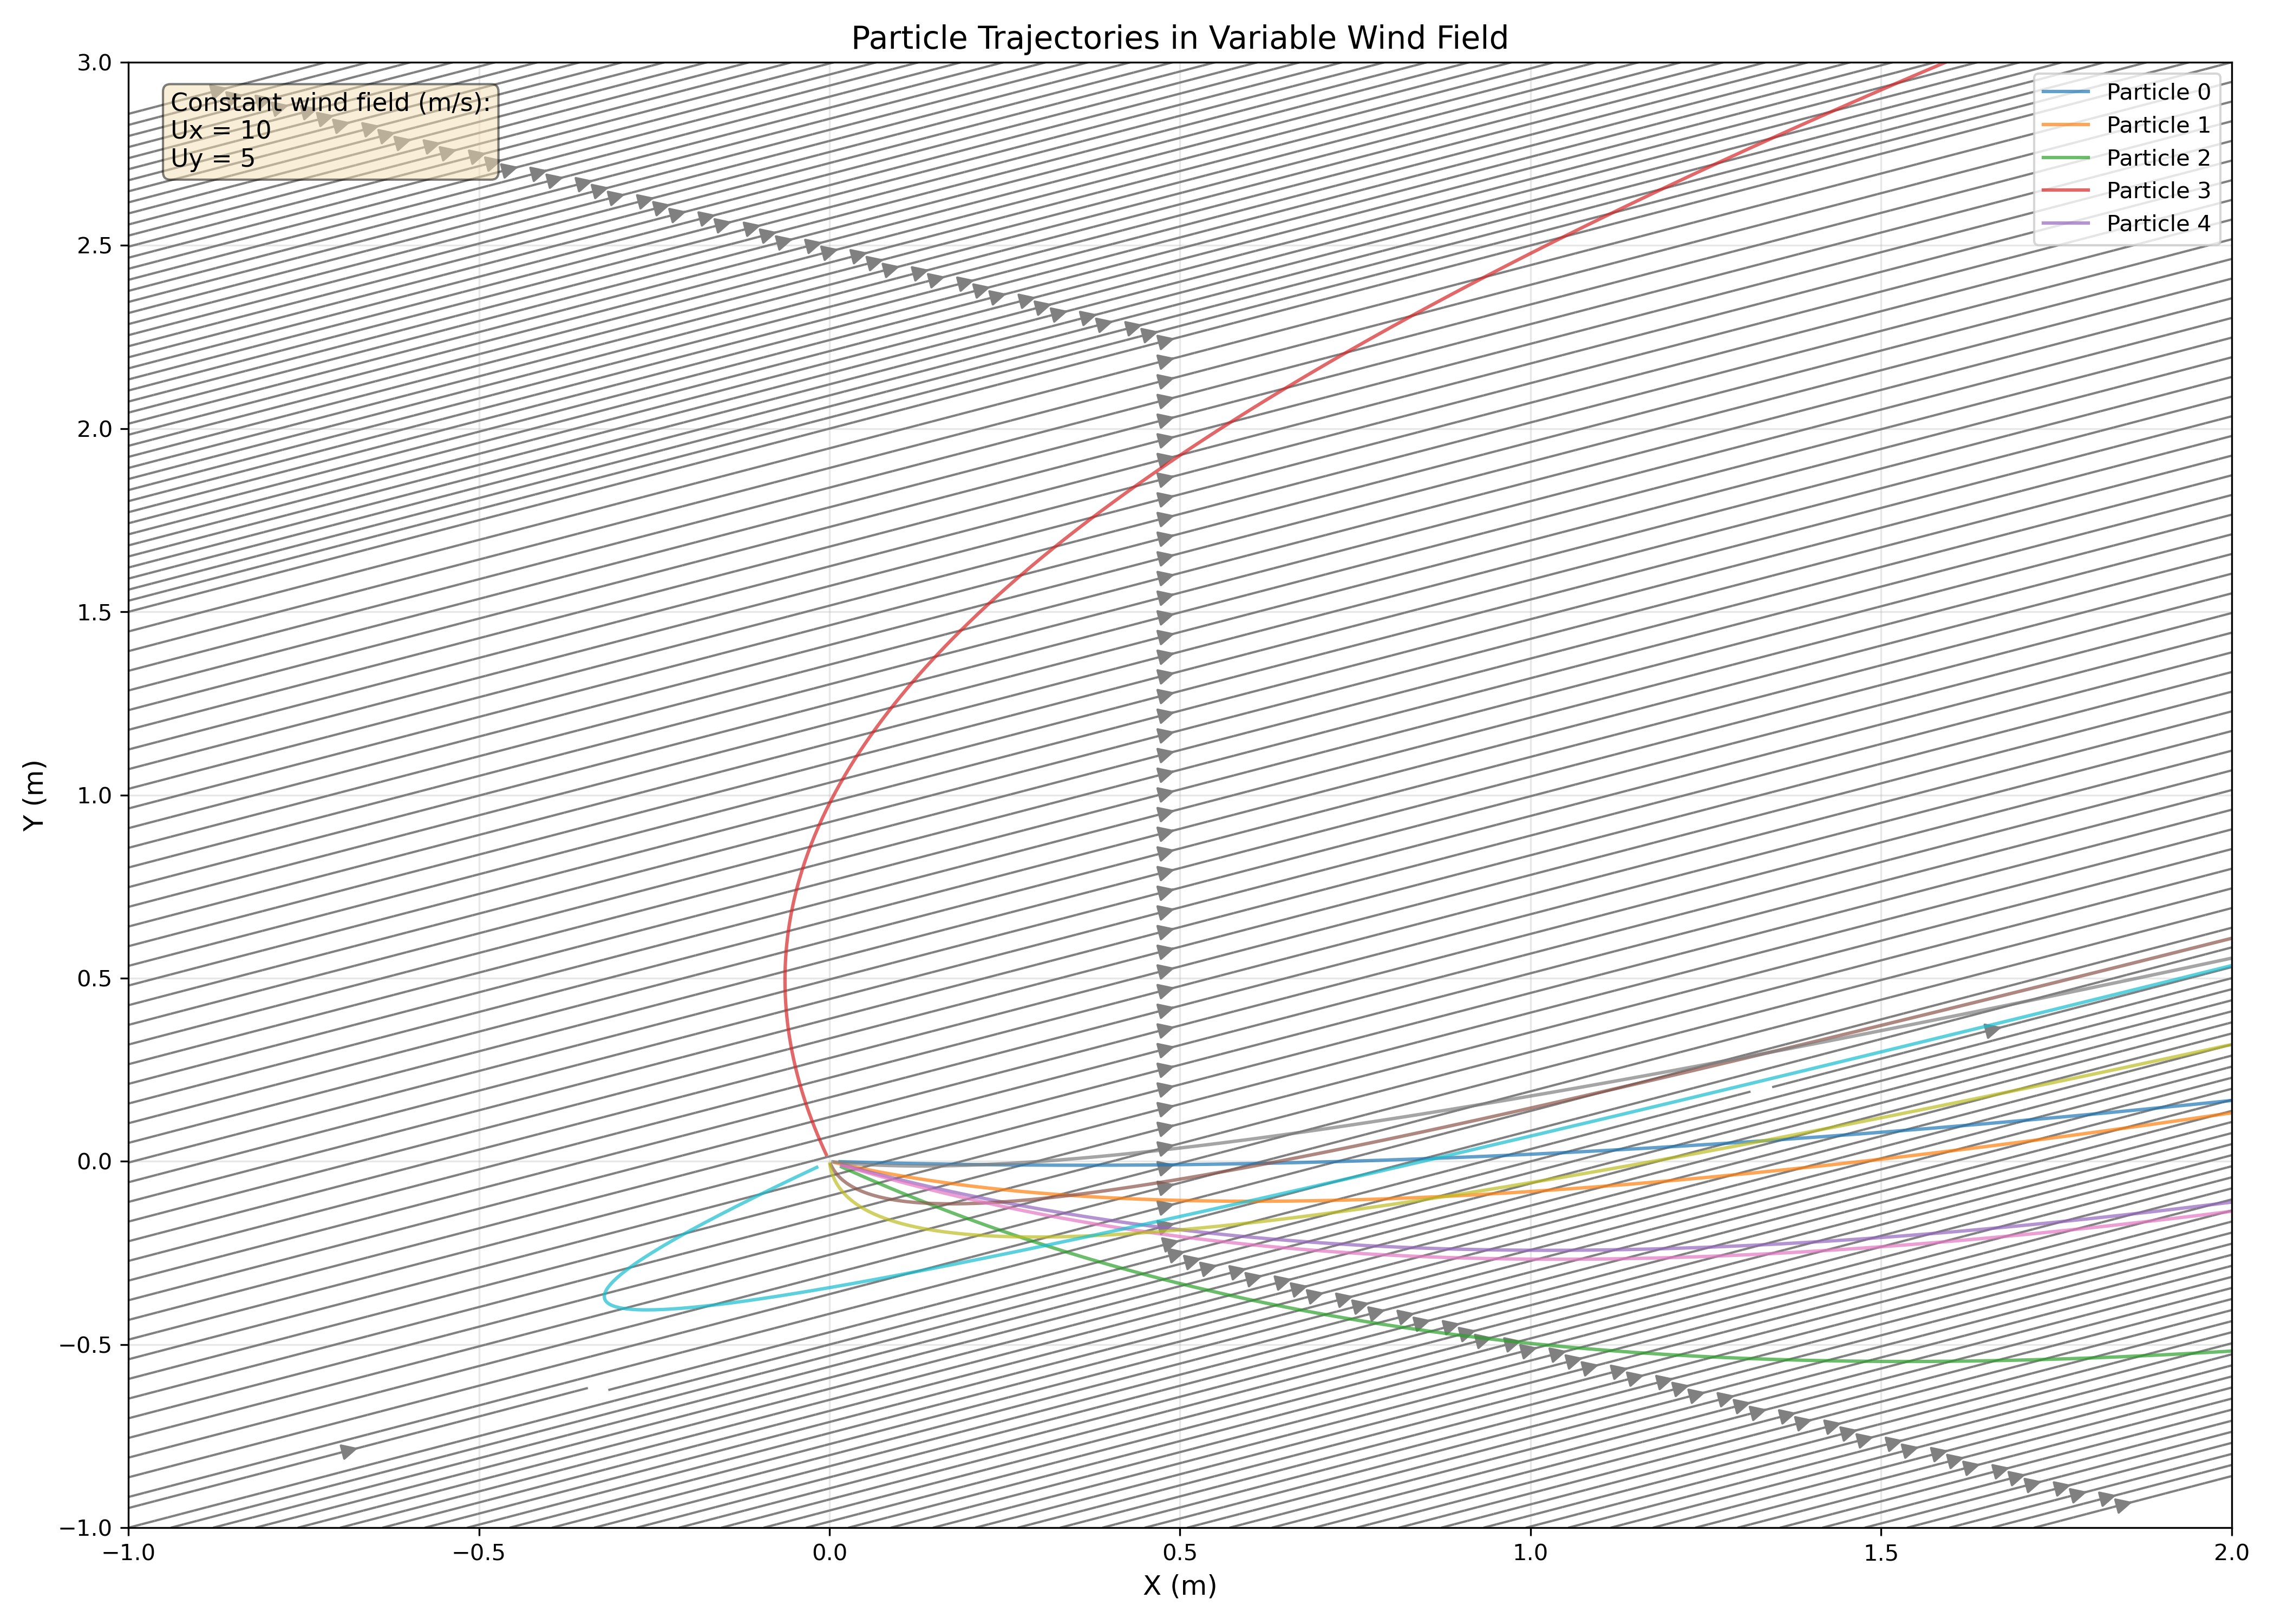
\includegraphics[width=0.8\textwidth]{wind_field_1_particles_10.png}
    \caption{Однородное поле, $N = 10$ частиц}
    \label{fig:field1_10}
\end{figure}

На рис.~\ref{fig:field1_10} видно, что в самом начале частицы движутся в разные
стороны из-за заданной начальной скорости. Со временем под действием ветра их скорости
и траектории постепенно меняются, приближаясь к траекториям линий тока.

\begin{figure}[!htbp]
    \centering
    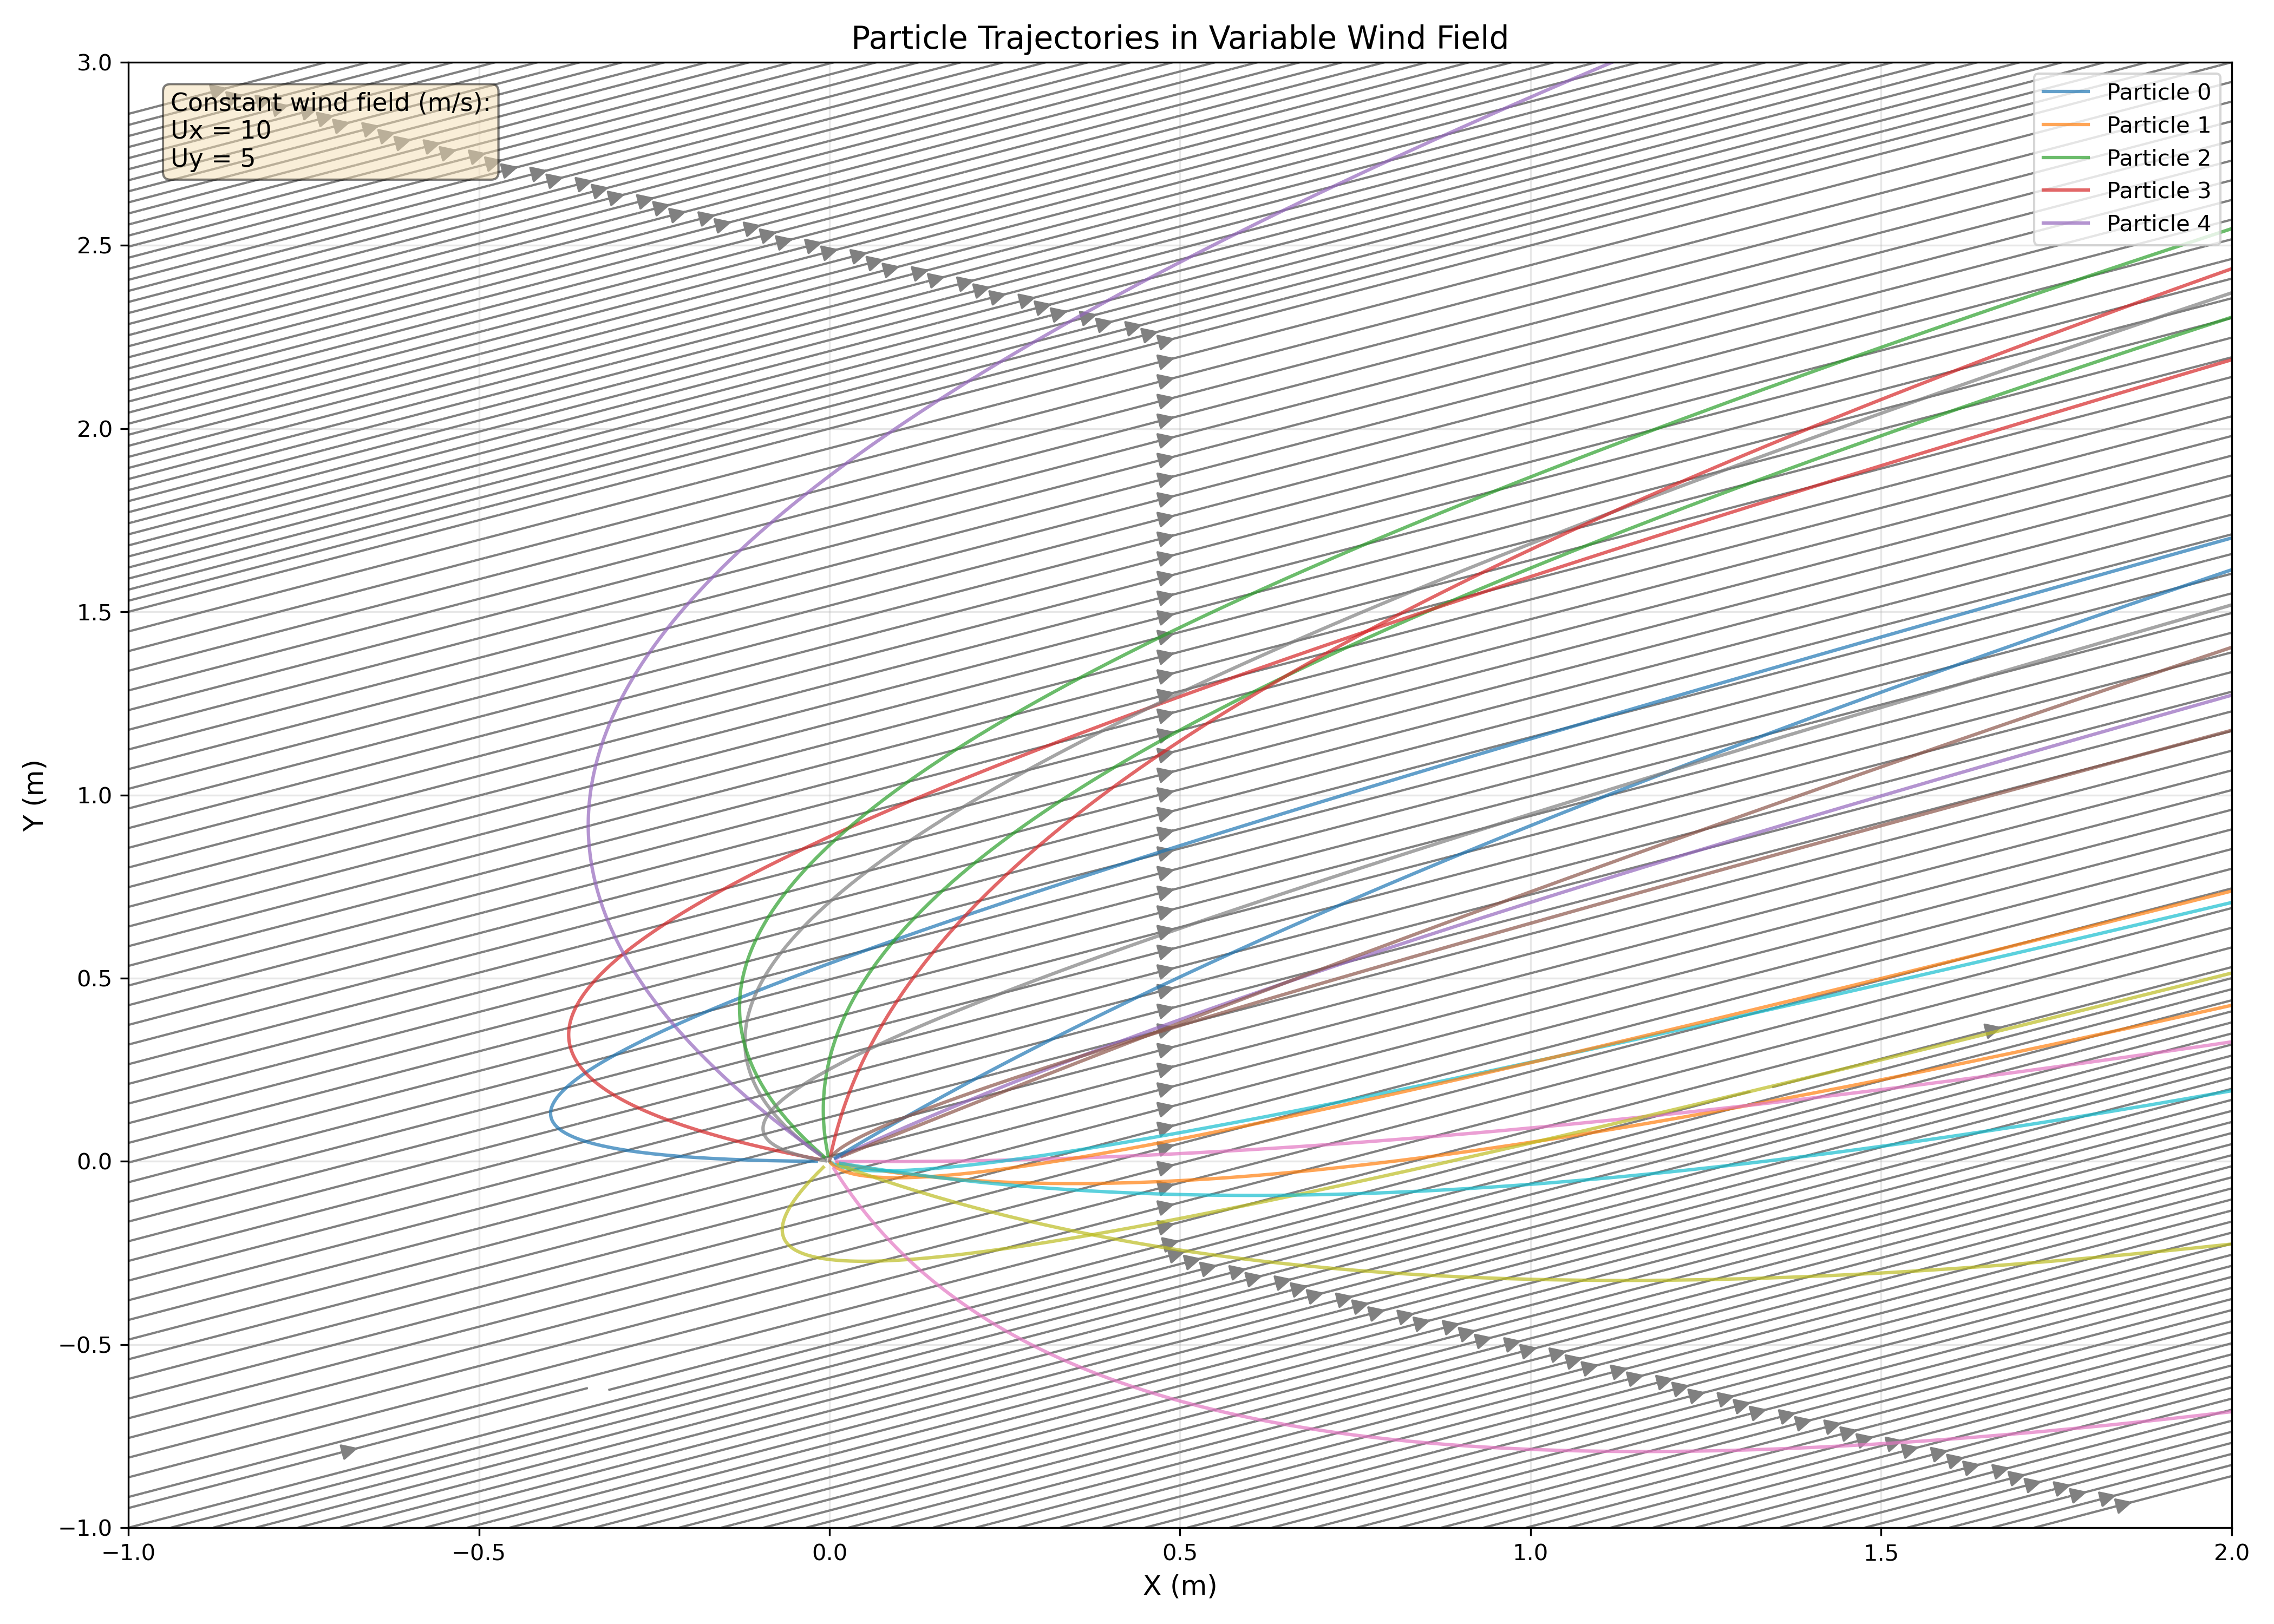
\includegraphics[width=0.8\textwidth]{wind_field_1_particles_20.png}
    \caption{Однородное поле, $N = 20$ частиц}
    \label{fig:field1_20}
\end{figure}

При увеличении числа частиц до $N = 20$ (рис.~\ref{fig:field1_20}) эта картина
видна ещё лучше. Сначала траектории заметно расходятся, так как частицы получают
разные начальные скорости. Потом ветер выравнивает их движение, и дальше почти все
кривые идут в одном и том же направлении.

\subsection{Переменное поле скорости~1 (поле~2)}

Поле задаётся формулами $u_x = 5 + y\sin(\pi y) + e^{-0{,}1x}$,
$u_y = 8 + 0{,}3x\sin(\pi y)$ и обладает периодической структурой по оси $y$
и экспоненциальным убыванием компоненты $u_x$ по оси $x$.

\begin{figure}[!htbp]
    \centering
    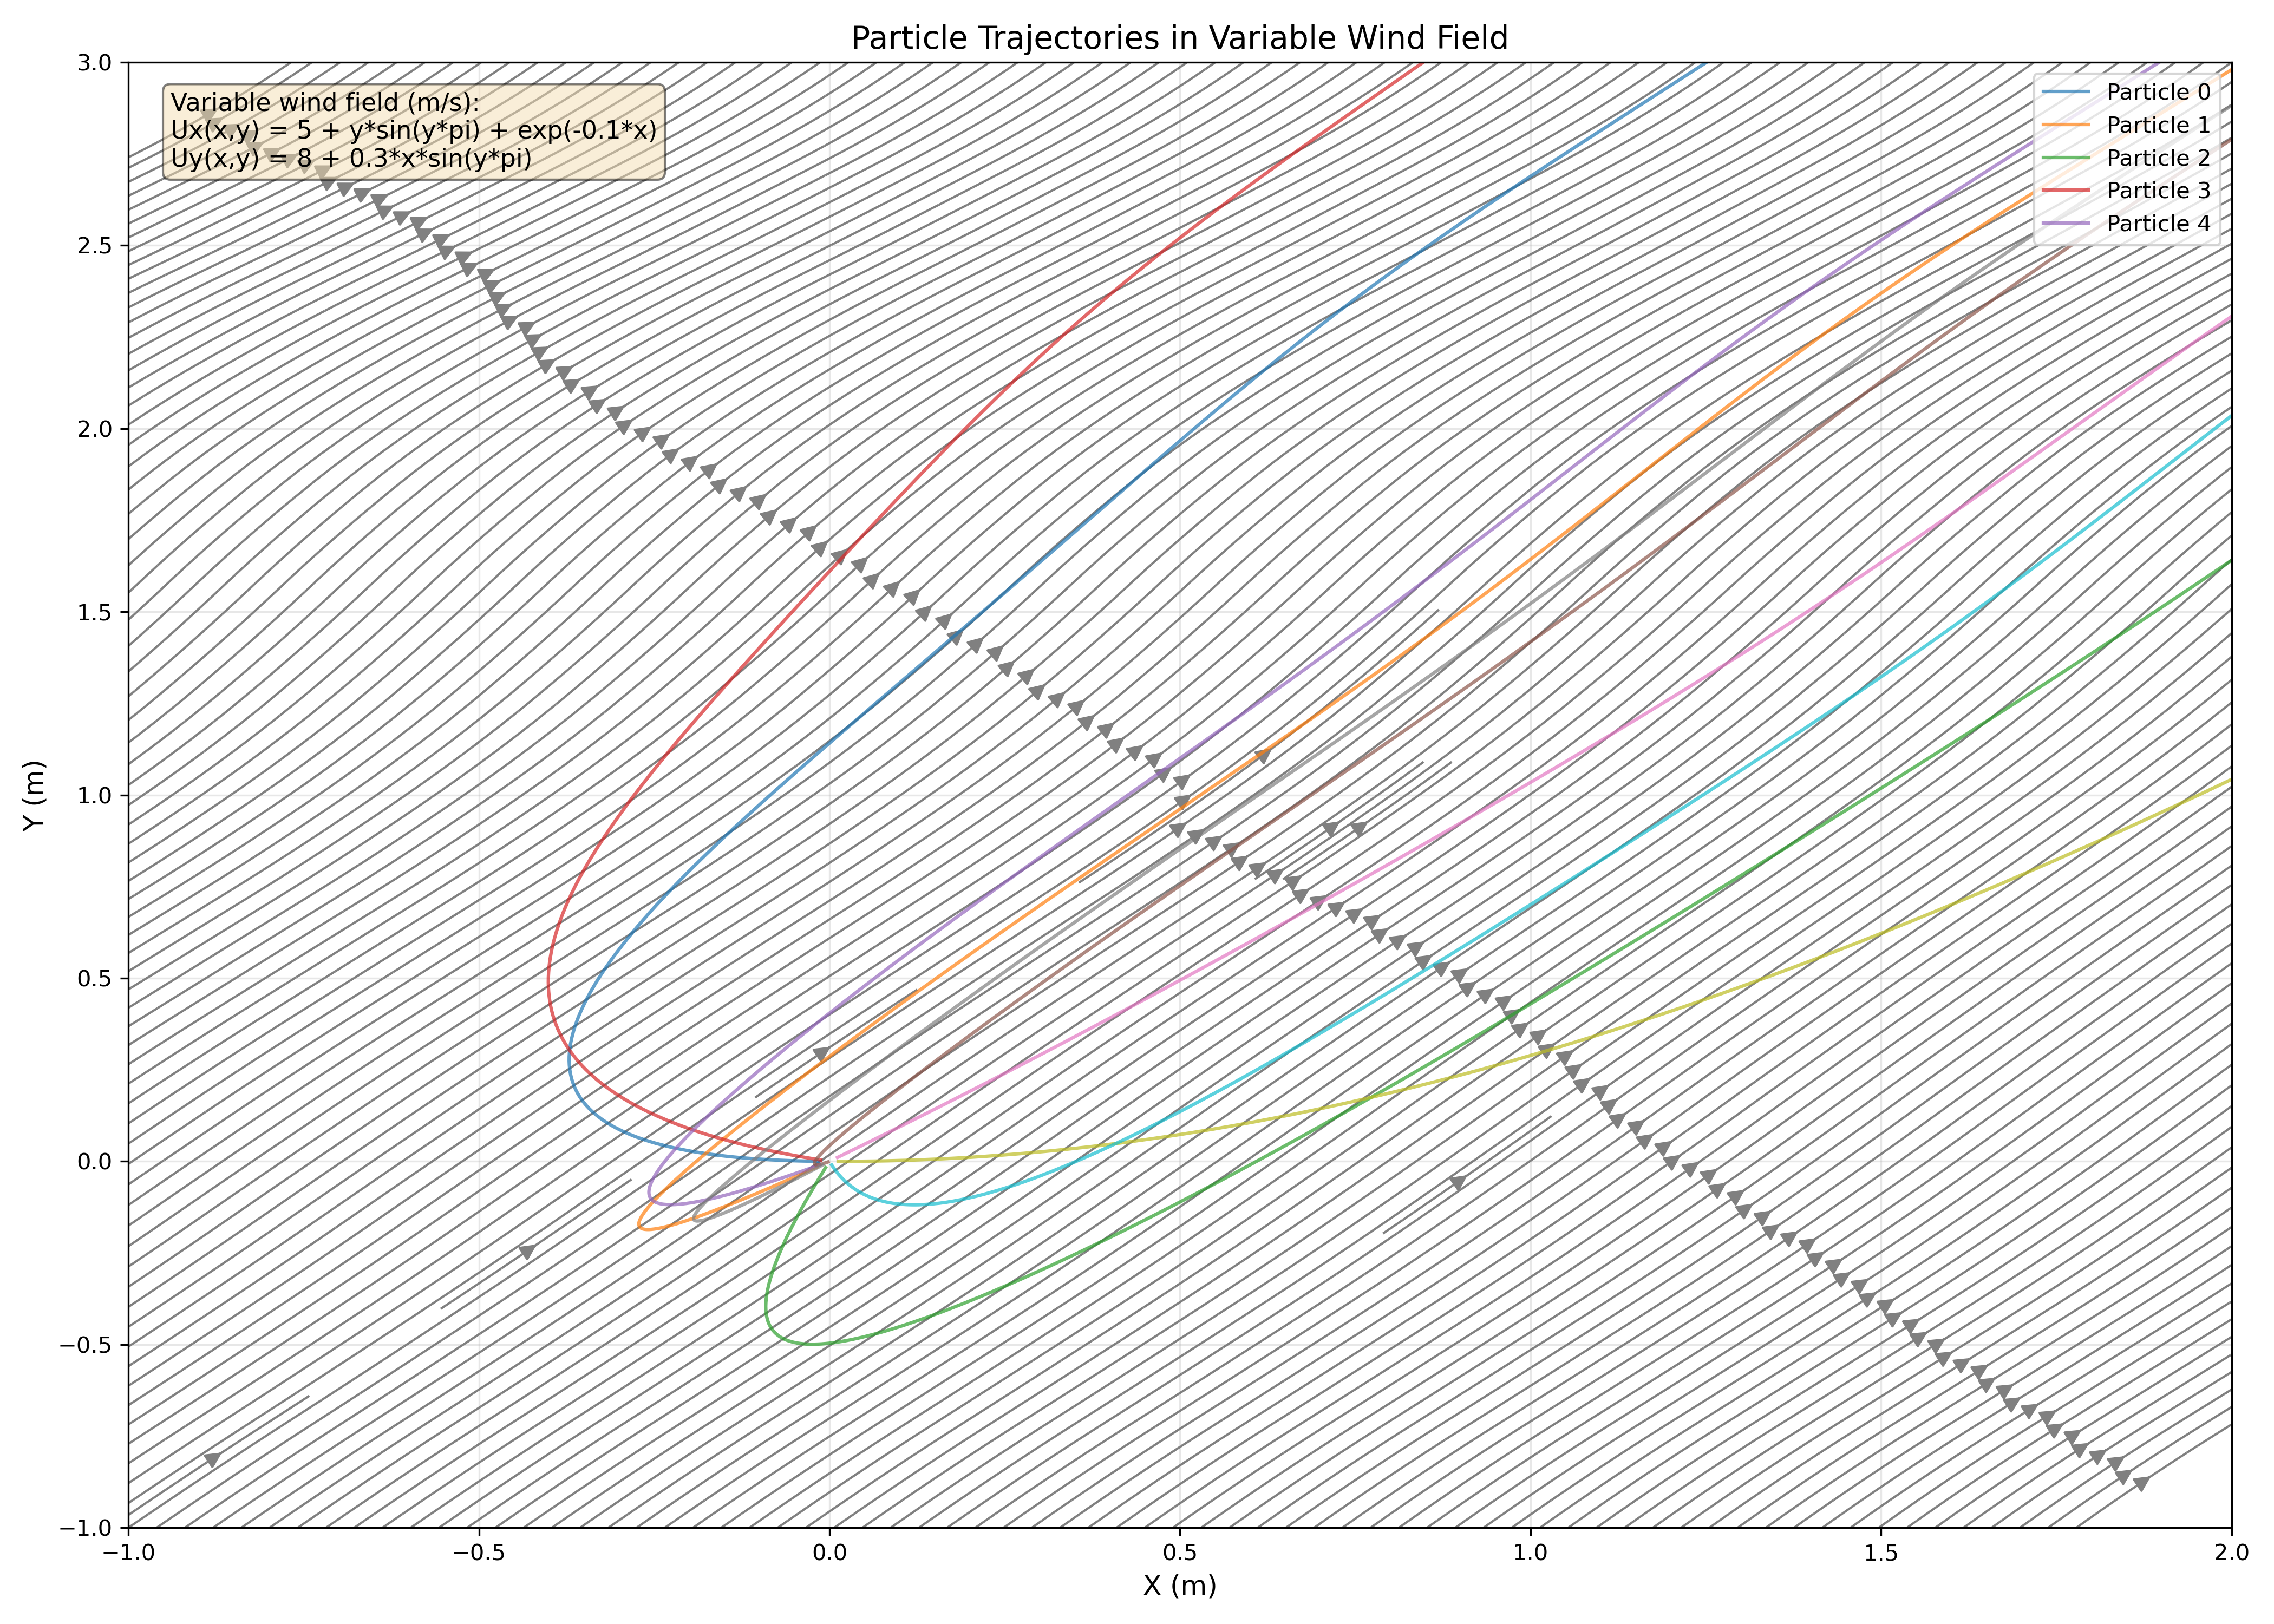
\includegraphics[width=0.8\textwidth]{wind_field_2_particles_10.png}
    \caption{Переменное поле~1, $N = 10$ частиц}
    \label{fig:field2_10}
\end{figure}

На рис.~\ref{fig:field2_10} сначала снова видно разлёт частиц из-за заданной
начальной скорости. Но дальше поток воздуха уже не просто сдувает их в одну сторону,
как в предыдущем случае, а ещё и по-разному изгибает траектории в зависимости
от того, где находилась частица в начальный момент времени.

\subsection{Переменное поле скорости~2 (поле~3)}

Поле задаётся формулами $u_x = x\cos(\pi y/2) + y + 5$,
$u_y = 10\sin(\pi y / 2)$ и обладает двумя горизонтальными линиями притяжения
при $y = \pm 2$, где $u_y = 0$ и знак $u_y$ меняется.
Здесь картина уже заметно отличается от предыдущих случаев: поток как будто
разделяет частицы на две группы --- верхнюю и нижнюю.

\begin{figure}[!htbp]
    \centering
    \includegraphics[width=0.8\textwidth]{wind_field_3_particles_10.png}
    \caption{Переменное поле~2, $N = 10$ частиц}
    \label{fig:field3_10}
\end{figure}

На рис.~\ref{fig:field3_10} после начального разлёта становится видно, что
частицы выше оси $x$ постепенно уходят вверх, а частицы ниже оси --- вниз.
Потом обе группы начинает сдувать вправо. Из-за этого траектории выглядят как
изогнутые крючки.

\begin{figure}[!htbp]
    \centering
    \includegraphics[width=0.8\textwidth]{wind_field_3_particles_20.png}
    \caption{Переменное поле~2, $N = 20$ частиц}
    \label{fig:field3_20}
\end{figure}

При $N = 20$ (рис.~\ref{fig:field3_20}) это разделение видно ещё лучше.
Часть частиц уходит в верхнюю полосу, часть --- в нижнюю, а потом обе группы
ветер тянет вправо. По сравнению с однородным полем путь до такого движения
получается длиннее и заметно сложнее.

\begin{figure}[!htbp]
    \centering
    \includegraphics[width=0.8\textwidth]{wind_field_3_particles_100.png}
    \caption{Переменное поле~2, $N = 100$ частиц}
    \label{fig:field3_100}
\end{figure}

Эксперимент с $N = 100$ (рис.~\ref{fig:field3_100}) показывает ту же картину,
но уже для большого числа частиц. Хорошо видно, что почти все траектории
собираются в две полосы: одну сверху и одну снизу. В середине частиц остаётся
заметно меньше. Это значит, что такое поле со временем разводит частицы в две
основные области.

\subsection{Вихревое поле и видеоэволюция плотности}

Для поля \textbf{U\_FUNCTION=4} в проекте дополнительно построен график
траекторий при $N = 20$ частицах. На рис.~\ref{fig:field4_20} видно,
что частицы начинают вращаться вокруг центра, постепенно удаляясь от центра
за счёт инерции. Их траектории идут по длинным дугам, и вместо простого
сноса вправо здесь получается закрученное движение.

\begin{figure}[!htbp]
    \centering
    \includegraphics[width=0.8\textwidth]{wind_field_4_particles_20.png}
    \caption{Вихревое поле, $N = 20$ частиц}
    \label{fig:field4_20}
\end{figure}

Для расширенных конфигураций \textbf{U\_FUNCTION=4,6,7,8,9} основным
инструментом анализа стала видеовизуализация плотности. В каталоге
\textbf{videos/} сохранены ролики \textbf{density\_200000\_f4.mp4},
\textbf{density\_2000\_f6.mp4}, \linebreak \textbf{density\_2000\_f7.mp4},
\textbf{density\_2000\_f8.mp4}, \textbf{density\_2000\_f9.mp4}
и другие. На рис.~\ref{fig:video_frames} приведены характерные кадры
из трёх сгенерированных видео.

\begin{figure}[!htbp]
    \centering
    \begin{minipage}[t]{0.45\textwidth}
        \centering
        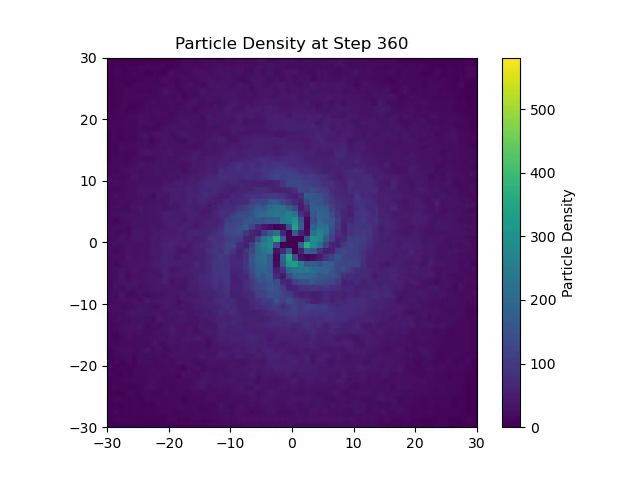
\includegraphics[width=\textwidth]{density_200000_f4_frame.png}
        \small Поле 4: спиральная структура плотности
    \end{minipage}
    \hfill
    \begin{minipage}[t]{0.45\textwidth}
        \centering
        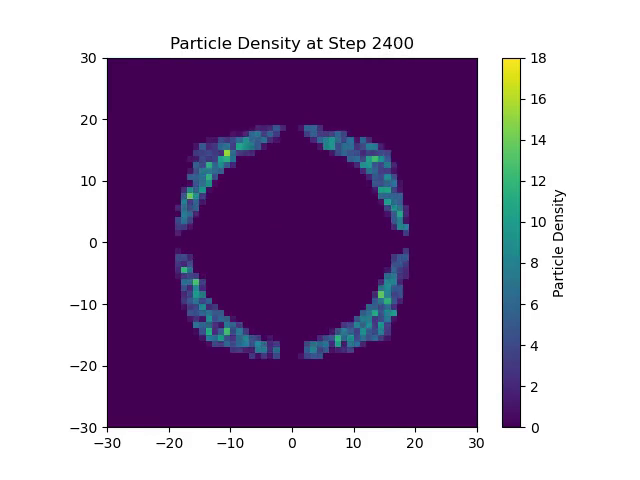
\includegraphics[width=\textwidth]{density_2000_f6_frame.png}
        \small Поле 6: формирование кольцевой зоны выноса
    \end{minipage}
    \hfill
    \begin{minipage}[t]{0.45\textwidth}
        \centering
        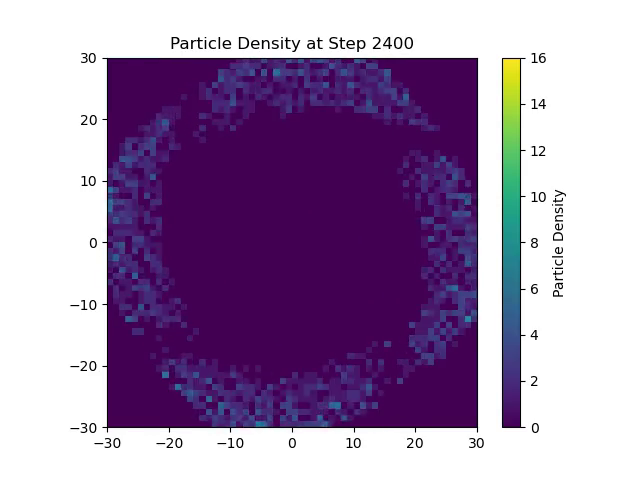
\includegraphics[width=\textwidth]{density_2000_f9_frame.png}
        \small Поле 9: кольцо с выносом по спирали
    \end{minipage}
    \caption{Кадры из сгенерированных видео плотности для различных полей скорости}
    \label{fig:video_frames}
\end{figure}

Кадр для поля~4 показывает, что плотность закручивается около центра. Для поля~6
частицы образуют сравнительно узкое кольцо и постепенно уходят от центра. Для
поля~9 тоже появляется кольцо, но оно выглядит менее ровным из-за дополнительного
вращения. Такие видео удобны тем, что по ним сразу видно поведение всей группы
частиц, а не только отдельных траекторий.

\subsection{Производительность программного комплекса}

Для оценки вычислительной эффективности реализации были проведены замеры
времени выполнения на двух конфигурациях. Результаты приведены в
таблице~\ref{tab:performance}.

\begin{table}[h]
\centering
\caption{Время выполнения симуляции и генерации видео}
\label{tab:performance}
\begin{tabular}{|l|r|r|r|}
\hline
\textbf{Этап} & \textbf{$N = 1\,000$} & \textbf{$N = 200\,000$} \\
\hline
Расчёт траекторий (C++)   & $\approx 7$~с   & $\approx 23$~мин \\
Сохранение плотности      & $\approx 2$~с   & $\approx 2$~с  \\
Генерация видео (Python)  & $\approx 17$~с  & $\approx 23$~с  \\
\hline
\textbf{Итого}            & $\approx 26$~с  & $\approx 23.5$~мин \\
\hline
\end{tabular}
\end{table}

При $N = 1\,000$ частицах полный цикл --- расчёт траекторий, сохранение
матриц плотности и генерация видео --- занял около 26~секунд.
Максимальная зафиксированная плотность составила 11~частиц на ячейку,
а итоговое видео при 30~FPS и 5000~кадрах имеет продолжительность около
167~секунд (2~мин 47~с).

При $N = 200\,000$ суммарное время работы составило около получаса.
Основная доля времени приходится на расчёт траекторий в C++: каждая из
$200\,000$ частиц проходит 5000~шагов метода Рунге--Кутты, что в совокупности
составляет $10^9$ вычислений правой части системы~\eqref{eq:system}.
Генерация видео при большом $N$ занимает примерно столько же времени,
поскольку скрипт \textbf{density\_video.py} работает с уже готовыми
матрицами плотности и не зависит от числа частиц.

Таким образом, узким местом производительности является цикл по частицам
в C++. При необходимости дальнейшего ускорения наиболее перспективным
направлением является распараллеливание цикла средствами \linebreak OpenMP, поскольку
траектории частиц вычисляются независимо друг от друга. Или же можно перенести рассчёты
на GPU с помощью CUDA или OpenCL, что может обеспечить ещё большую скорость выполнения
при больших $N$.

\subsection{Общие выводы по результатам экспериментов}

Проведённые численные эксперименты позволяют сделать несколько простых выводов.

На первых шести рисунках частицы сначала разлетаются из-за заданной начальной
скорости. Затем движение всё сильнее определяется полем скорости воздуха,
и поток воздуха начинает менять траектории в соответствии со своей формой.

В однородном поле частицы со временем начинают двигаться почти в одном
направлении. В более сложных полях траектории изгибаются сильнее, а сами
частицы могут разделяться на группы. Особенно хорошо это видно в поле~3,
где одна часть частиц уходит вверх, а другая вниз.

Если увеличить число частиц, общая картина не меняется, но становится проще
увидеть, где именно частицы собираются чаще, а где их почти нет.

%%%%%%%%%%%%%%%%%%%%%%%%%%%%%%%%%%%%%%%%%%%%%%%%%%%%%%%%%%%%%%%%%%%%%%%%%%%%%%%%%%%%%%%%%%%%%%%%%%%%%%%%%%%
%%%%%%%%%%%%%%%%%%%%%%%%%%%%%%%%%%%%%%%%%%%%%%%%%%%%%%%%%%%%%%%%%%%%%%%%%%%%%%%%%%%%%%%%%%%%%%%%%%%%%%%%%%%

\FloatBarrier
\clearpage
\section*{ЗАКЛЮЧЕНИЕ}
\addcontentsline{toc}{section}{ЗАКЛЮЧЕНИЕ}

Выполненная работа была посвящена разработке программы для
численного моделирования движения дисперсных частиц в потоке воздуха методом
частиц. Поставленная цель была достигнута: создана программа, которая позволяет
задавать различные поля скорости несущей фазы, рассчитывать траектории большого
количества частиц, строить распределения плотности и выполнять визуализацию
результатов как в виде отдельных графиков, так и в виде видеоряда.

В теоретической части работы была выбрана лагранжева постановка задачи, в которой
каждая частица рассматривается как отдельный материальный объект, движение которого
описывается системой обыкновенных дифференциальных уравнений. Такой подход позволяет
напрямую отслеживать траекторию каждой частицы, её скорость и реакцию на изменение
локального поля скорости несущей фазы.
Для численного интегрирования был использован метод Рунге--Кутты четвёртого порядка,
который обеспечивает достаточную точность при разумной вычислительной стоимости и
хорошо подходит для большого числа независимых траекторий.

Практическим результатом стала реализация вычислительного ядра на языке C++17.
В программе реализованы вычисление числа Рейнольдса, пересчёт коэффициента
аэродинамического сопротивления и интегрирование движения частиц в десяти различных
полях скорости несущей фазы. Такое расширение набора полей по сравнению с более ранней
версией проекта позволило перейти от анализа нескольких базовых сценариев к исследованию
широкого класса течений: однородных, неоднородных, вихревых, радиальных и составных.
Тем самым программный комплекс стал заметно более универсальным и пригодным для
постановки новых вычислительных экспериментов.

Важной частью работы стала возможность постобработки результатов. Для анализа траекторий частиц
был подготовлен Python-скрипт, строящий линии тока и индивидуальные траектории
частиц. Для анализа общего поведения дисперсной фазы реализовано накопление
плотности на фиксированной сетке и генерация видео эволюции плотности.

Проведённые численные эксперименты показали, что характер движения дисперсной фазы
определяется структурой поля скорости несущей фазы. В однородном потоке частицы
после переходного режима стремятся к движению вдоль линий тока. В неоднородных полях
наблюдаются асимметричные петли траекторий и перераспределение частиц по различным зонам
течения. В вихревых и радиально-вихревых конфигурациях возникает качественно иная картина:
частицы начинают образовывать кольцевые, спиральные и закрученные структуры.

Результаты вычислительных экспериментов также позволили оценить производительность созданного
программного комплекса. При умеренном числе частиц программа подходит для быстрого анализа
траекторий и отладки параметров, а при больших значениях $N$ позволяет исследовать уже
общее поведение облака. Основная вычислительная нагрузка приходится на цикл по
частицам в C++-части программы, тогда как этапы визуализации и формирования видеоряда играют
вспомогательную, хотя и важную, роль. Это указывает на понятное направление дальнейшего развития
проекта: распараллеливание вычислений и оптимизация хранения результатов.

Таким образом, разработанный программный комплекс можно рассматривать как законченную основу
для дальнейшего исследования динамики дисперсных частиц в заданных воздушных потоках. Он уже
позволяет проводить качественный и количественный анализ, сравнивать различные поля скорости,
строить графические и видеоиллюстрации, а также масштабировать расчёт под разные сценарии.
Перспективами развития работы являются учёт дополнительных физических факторов, таких как
гравитация, теплообмен, взаимодействие частиц между собой, а также расширение библиотеки полей
скорости и применение параллельных вычислений для ускорения расчётов.

%%%%%%%%%%%%%%%%%%%%%%%%%%%%%%%%%%%%%%%%%%%%%%%%%%%%%%%%%%%%%%%%%%%%%%%%%%%%%%%%%%%%%%%%%%%%%%%%%%%%%%%%%%%
%%%%%%%%%%%%%%%%%%%%%%%%%%%%%%%%%%%%%%%%%%%%%%%%%%%%%%%%%%%%%%%%%%%%%%%%%%%%%%%%%%%%%%%%%%%%%%%%%%%%%%%%%%%

\FloatBarrier
\clearpage
\section*{ПРИЛОЖЕНИЯ}
\addcontentsline{toc}{section}{ПРИЛОЖЕНИЯ}

\subsection*{Приложение А. Основные определения полей скорости}

Ниже приведён ключевой фрагмент модуля \textbf{constants.cpp}, в котором задаются
несколько характерных полей скорости несущей фазы. Именно через этот механизм
осуществляется переключение между различными режимами численного эксперимента.

\begin{lstlisting}[style=diplomacode,language=C++,caption={Фрагмент файла constants.cpp: задания нескольких полей скорости}]
#if U_FUNCTION == 1
    pos U_AIR(double x, double y) {
        return {10.0, 5.0};
    }
#endif

#if U_FUNCTION == 4
    pos U_AIR(double x, double y) {
        double Ux = -sqrt(x*x + y*y) * y;
        double Uy =  sqrt(x*x + y*y) * x;
        return {Ux, Uy};
    }
#endif

#if U_FUNCTION == 9
    pos U_AIR(double x, double y) {
        double dx = x, dy = y;
        double r = sqrt(dx*dx + dy*dy) + 1e-6;

        double Vr = 8.0;
        double Vt = 5.0;

        double urx = dx / r, ury = dy / r;
        double utx = -dy / r, uty = dx / r;

        return {Vr*urx + Vt*utx, Vr*ury + Vt*uty};
    }
#endif
\end{lstlisting}

\subsection*{Приложение Б. Правая часть системы для частицы}

Следующий фрагмент показывает, как в классе \textbf{Particle} вычисляются
относительная скорость, число Рейнольдса, коэффициент сопротивления и правая
часть системы ОДУ для дальнейшего интегрирования.

\begin{lstlisting}[style=diplomacode,language=C++,caption={Фрагмент файла particle.cpp: вычисление правой части системы движения частицы}]
void particleSystem(const state_type &y, state_type &dydt, double t) {
    double qx = y[0];
    double qy = y[1];
    double vx = y[2];
    double vy = y[3];
    auto [ ux, uy ] = U_AIR(qx, qy);

    norma = sqrt(pow(ux - vx, 2) + pow(uy - vy, 2));
    Re = (2 * RO_AIR * norma * radius) / Myu;
    Cd = pow(0.325 + sqrt(0.124 + 24 / Re), 2);

    double K = M_PI*radius*radius/2 * Cd * RO_AIR / mass;
    dydt[0] = vx;
    dydt[1] = vy;
    dydt[2] = K * norma * (ux - vx);
    dydt[3] = K * norma * (uy - vy);
}
\end{lstlisting}

\subsection*{Приложение В. Основной цикл накопления плотности}

Вычислительное ядро программы последовательно обрабатывает все частицы,
получает их траектории и одновременно накапливает число частиц в ячейках
пространственной сетки. Именно этот участок отвечает за формирование данных,
по которым затем строятся тепловые карты и видео.

\begin{lstlisting}[style=diplomacode,language=C++,caption={Фрагмент файла main.cpp: цикл по частицам и накопление плотности}]
for (int i = 0; i < NUM_PARTICLES; i++) {
    double x = (1 + (rand() % 100) / 10.0) * (rand() % 2 == 0 ? 1 : -1);
    double y = (1 + (rand() % 100) / 10.0) * (rand() % 2 == 0 ? 1 : -1);
    double Vx = 0;
    double Vy = 0;

    particles[i] = Particle(x, y, Vx, Vy);
    pair<vector<pos>, vector<pos>> trajectory =
        particles[i].calclulateTrajectory(STEPS);

    for (int k = 0; k < trajectory.first.size(); k++) {
        int shift_coef = 30;
        int i = floor(trajectory.first[k].y) + shift_coef;
        int j = floor(trajectory.first[k].x) + shift_coef;
        if (0 > i || i >= 60 || 0 > j || j >= 60) continue;

        q_squares[i][j][k] = q_squares[i][j][k] + 1;
        if (q_squares[i][j][k] > MAX_Q) MAX_Q = q_squares[i][j][k];
    }
}
\end{lstlisting}

%%%%%%%%%%%%%%%%%%%%%%%%%%%%%%%%%%%%%%%%%%%%%%%%%%%%%%%%%%%%%%%%%%%%%%%%%%%%%%%%%%%%%%%%%%%%%%%%%%%%%%%%%%%
%%%%%%%%%%%%%%%%%%%%%%%%%%%%%%%%%%%%%%%%%%%%%%%%%%%%%%%%%%%%%%%%%%%%%%%%%%%%%%%%%%%%%%%%%%%%%%%%%%%%%%%%%%%

\newpage
\begingroup
\addcontentsline{toc}{section}{СПИСОК ЛИТЕРАТУРЫ}
\begin{thebibliography}{9}
\setlength{\itemsep}{0.2em}
\setlength{\parskip}{0pt}

\bibitem{Nigmatulin1978}
Нигматулин~Р.И.
\textit{Основы механики гетерогенных сред}.
--- М.: Наука, 1978. --- 336~с.

\bibitem{Nigmatulin1987}
Нигматулин~Р.И.
\textit{Динамика многофазных сред}. Ч.~1.
--- М.: Наука, 1987. --- 464~с.

\bibitem{HairerRK}
Бахвалов~Н.С., Жидков~Н.П., Кобельков~Г.М.
\textit{Численные методы} : учебник.
--- 9-е изд. --- М. : Лаборатория знаний, 2020. --- 636~с.

\bibitem{BoostOdeint}
Ahnert~K., Mulansky~M.
Odeint~--- Solving ordinary differential equations in C++~//
\textit{AIP Conference Proceedings}.
--- 2011. --- Vol.~1389. --- P.~1586--1589.

\bibitem{SchillerNaumann1935}
Schiller~L., Naumann~A.
A drag coefficient correlation~//
\textit{Zeitschrift des Vereins Deutscher Ingenieure}.
--- 1935. --- Vol.~77. --- P.~318--320.

\bibitem{CroweMultiphase}
Crowe~C.T., Schwarzkopf~J.D., Sommerfeld~M., Tsuji~Y.
\textit{Multiphase Flows with Droplets and Particles}.
--- 2nd~ed. --- Boca~Raton: CRC Press, 2012. --- 509~p.

\bibitem{BoostLibrary}
Boost C++ Libraries [Электронный ресурс].
--- URL: \textbf{https://www.boost.org} (дата обращения: 01.03.2026).

\bibitem{Matplotlib}
Hunter~J.D.
Matplotlib: A 2D graphics environment~//
\textit{Computing in Science \& Engineering}.
--- 2007. --- Vol.~9, No.~3. --- P.~90--95.

\bibitem{NumPy}
Harris~C.R. et~al.
Array programming with NumPy~//
\textit{Nature}.
--- 2020. --- Vol.~585. --- P.~357--362.

\bibitem{FFmpeg}
FFmpeg [Электронный ресурс].
--- URL: \textbf{https://ffmpeg.org} (дата обращения: 01.03.2026).

\bibitem{PythonDotenv}
python-dotenv [Электронный ресурс].
--- URL: \textbf{https://github.com/theskumar/python-dotenv}
(дата обращения: 01.03.2026).
\end{thebibliography}
\endgroup

\end{document}